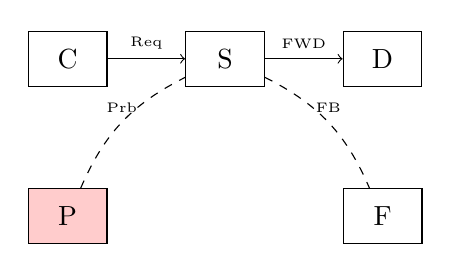
\begin{tikzpicture}[
    scale=0.4, % Further reduced scale
    node distance=2cm, % Further reduced distance
    % user/.style={circle,draw,minimum size=0.6cm},
    % attacker/.style={rectangle,draw,fill=red!20,minimum width=1cm,minimum height=0.7cm},
    % server/.style={rectangle,draw,minimum width=1cm,minimum height=0.7cm}
    censor/.style={rectangle,draw,fill=red!20,minimum width=1cm,minimum height=0.7cm},
    proxy/.style={rectangle,draw,minimum width=1cm,minimum height=0.7cm},
    client/.style={rectangle,draw,minimum width=1cm,minimum height=0.7cm},
    destination/.style={rectangle,draw,minimum width=1cm,minimum height=0.7cm},
    webserver/.style={rectangle,draw,minimum width=1cm,minimum height=0.7cm}
]
    % Define nodes with shorter labels
    % \node[user] (alice) {A};
    % \node[attacker] (mitm) [right of=alice] {M};
    % \node[server] (server) [right of=mitm] {S};
    \node[client] (client) {C};
    \node[censor] (censor) [below of=client] {P};
    \node[proxy] (proxy) [right of=client] {S};
    \node[destination] (destination) [right of=proxy] {D};
    \node[webserver] (webserver) [below of=destination] {F};

    % Shorter arrows and smaller labels
    % \draw[->,thick] (alice) to[bend left=20] node[above,font=\tiny] {Msg} (mitm);
    % \draw[->,thick] (mitm) to[bend left=20] node[above,font=\tiny] {Mod} (server);
    % \draw[->,thick] (server) to[bend left=20] node[below,font=\tiny] {Rsp} (mitm);
    % \draw[->,thick] (mitm) to[bend left=20] node[below,font=\tiny] {Mod} (alice);
    \draw[->] (client) to node[above, font=\tiny] {Req} (proxy);
    \draw[dashed] (censor) to[bend left=20] node[above, font=\tiny] {Prb} (proxy);
    \draw[->] (proxy) to node[above, font=\tiny] {FWD} (destination);
    \draw[dashed] (proxy) to[bend left=20] node[above, font=\tiny] {FB} (webserver);
\end{tikzpicture}